\subsection{Hardware - V1.1}

    The switch module allows to switch 230V devices on and off and measure the current draw. 
    This module can not be compined with any other module. The switch module has two revisions,
    V1.0 and V1.1.

    Following components are required to fulfill the requirements:

    \begin{itemize}
        \item 1. Power-Supply
        \item 2. Switch
        \item 3. Current-Sensor
     
    \end{itemize}

    \subsubsection{Power-Supply}

        Because the switch module is switching 230V, it will also supplay itself with this voltage.
        A tranformer was chosen over a switching power supply because of the lower cost and the
        lower complexity.

        The used Transformer is from PLACEHOLDER with the type FL4/9 it has two 115V primary windings and
        two 9V secondary windings. The primary windings are connected in serial to the 230V mains and the
        secondary windings are connected in serial to the rectifier.

        The rectifier is a full-wave rectifier with a capacitor to smooth the output.

        \begin{figure}[H]
            \centering
            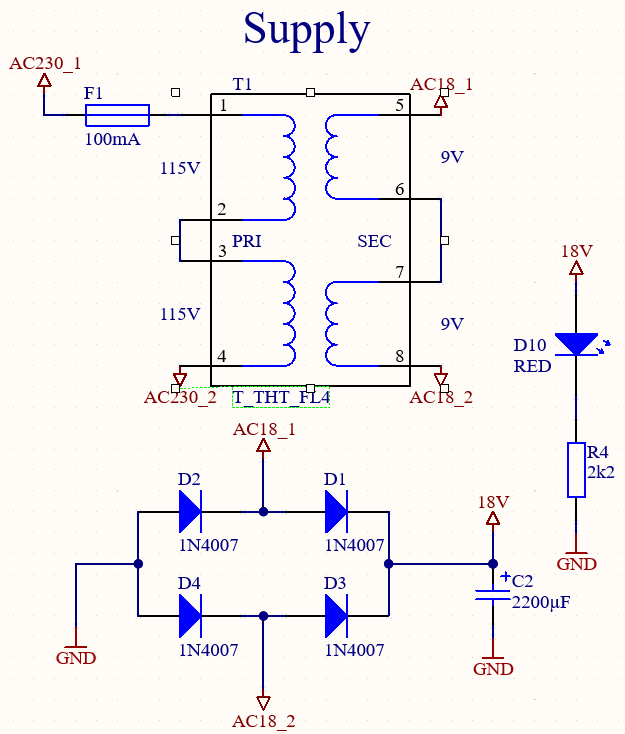
\includegraphics[width=0.5\textwidth]{assets/HW/Power-Supply-schematic.png}
            \caption{Power-Supply implemented in the schematic.}
        \end{figure}
        
        The output capacitor is calculated with the following formula:

        \begin{equation}
            C = \frac{I \cdot T}{\Delta U}
        \end{equation}

    \subsubsection{Relay}
        The switch module uses a relay to switch the 230V devices on and off. The relay used is 
        the JW1aFSN from Panasonic. The relay is controlled by a transistor and a flyback diode
        to protect the transistor from the voltage spike when the relay is switched off. The relay
        is rated for 10A at 250VAC.

        \begin{figure}[H]
            \centering
            
\includegraphics[width=0.8\textwidth]{assets/HW/TBD.png}
            \caption{Switch implemented in the schematic.}
        \end{figure}
    
    \subsubsection{Current-Sensor}

        The current sensor is used to measure the current draw of the switched device. The current
        sensor used is the ACS712ELCTR-20A-S from Allegro. The sensor is rated for 20A and has a sensitivity of 
        100mV/A. The sensor is connected to the microcontroller over an analog pin.

        The available versions of the sensor were +-5A, +-20A, and +-30A. The 20A version was 
        chosen because it covers the current range of the relay.

        
        

        \begin{figure}[H]
            \centering
            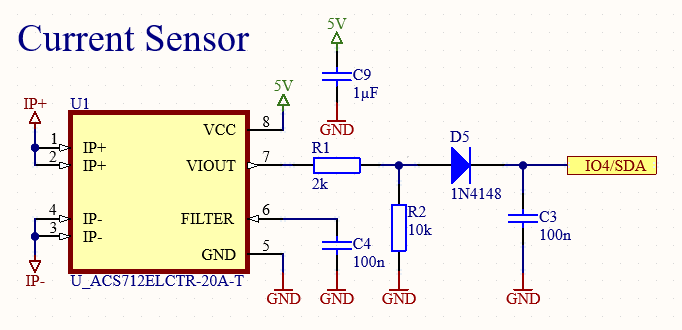
\includegraphics[width=0.8\textwidth]{assets/HW/Current-Sensor-schematic.png}
            \caption{Current-Sensor implemented in the schematic as shown in the datasheet \cite{}.}
        \end{figure}